%%%%%%%%%%%%%%%%%%%%%%%%%%%%%%%%%%%%%%%%%
% Sullivan Business Report
% LaTeX Template
% Version 1.0 (May 5, 2022)
%
% This template originates from:
% https://www.LaTeXTemplates.com
%
% Author:
% Vel (vel@latextemplates.com)
%
% License:
% CC BY-NC-SA 4.0 (https://creativecommons.org/licenses/by-nc-sa/4.0/)
%
%%%%%%%%%%%%%%%%%%%%%%%%%%%%%%%%%%%%%%%%%


%----------------------------------------------------------------------------------------
%	CLASS, PACKAGES AND OTHER DOCUMENT CONFIGURATIONS
%----------------------------------------------------------------------------------------

\documentclass[
    a4paper, % Paper size, use either a4paper or letterpaper
	12pt, % Default font size, the template is designed to look good at 12pt so it's best not to change this
	%unnumberedsections, % Uncomment for no section numbering
    ]{CSSullivanBusinessReport}
    
    \addbibresource{sample.bib} % BibLaTeX bibliography file

%----------------------------------------------------------------------------------------
%	REPORT INFORMATION
%----------------------------------------------------------------------------------------

\reporttitle{CPE 233 Hardware Assignment 7} % The report title is to appear on the title page and page headers, do not create manual new lines here as this will carry over to page headers

\reportsubtitle{Assembeling the Otter Wrapper} % Report subtitle, include new lines if needed

\reportauthors{Report by:\\\smallskip Ethan Vosburg (evosburg@calpoly.edu)} % Report authors/group/department, include new lines if needed

\reportdate{\today} % Report date, include new lines for additional information if needed

\rightheadercontent{
\includegraphics[width=3cm]{creodocs_logo.pdf}} % The content in the right header, you may want to add your own company logo or use your company/department name or leave this command empty for no right header content

%----------------------------------------------------------------------------------------

\begin{document}

%----------------------------------------------------------------------------------------
%	TITLE PAGE
%----------------------------------------------------------------------------------------

\thispagestyle{empty} % Suppress headers and footers on this page

\begin{fullwidth} % Use the whole page width
	\vspace*{-0.075\textheight} % Pull logo into the top margin
	
	\hfill
\includegraphics[width=5cm]{creodocs_logo.pdf} % Company logo

	\vspace{0.15\textheight} % Vertical whitespace

	\parbox{0.9\fulltextwidth}{\fontsize{50pt}{52pt}\selectfont\raggedright\textbf{\reporttitle}\par} % Report title, intentionally at less than full width for nice wrapping. Adjust the width of the \parbox and the font size as needed for your title to look good.
	
	\vspace{0.03\textheight} % Vertical whitespace
	
	{\LARGE\textit{\textbf{\reportsubtitle}}\par} % Subtitle
	
	\vfill % Vertical whitespace
	
	{\Large\reportauthors\par} % Report authors, group or department
	
	\vfill\vfill\vfill % Vertical whitespace
	
	{\large\reportdate\par} % Report date
\end{fullwidth}

\newpage

%----------------------------------------------------------------------------------------
%	DISCLAIMER/COPYRIGHT PAGE
%----------------------------------------------------------------------------------------

% \thispagestyle{empty} % Suppress headers and footers on this page

% \begin{twothirdswidth} % Content in this environment to be at two-thirds of the whole page width
% 	\footnotesize % Reduce font size
	
% 	\subsection*{Disclaimer}

% 	Lorem ipsum dolor sit amet, consectetur adipiscing elit. Praesent porttitor arcu luctus, imperdiet urna iaculis, mattis eros. Pellentesque iaculis odio vel nisl ullamcorper, nec faucibus ipsum molestie. Sed dictum nisl non aliquet porttitor. Etiam vulputate arcu dignissim, finibus sem et, viverra nisl. Aenean luctus congue massa, ut laoreet metus ornare in. Nunc fermentum nisi imperdiet lectus tincidunt vestibulum at ac elit.
	
% 	\subsection*{Copyright}
	
% 	\textcopyright~[Year] [Company] 
	
% 	Copyright notice text\ldots In hac habitasse platea dictumst. Curabitur mattis elit sit amet justo luctus vestibulum. In hac habitasse platea dictumst. Pellentesque lobortis justo enim, a condimentum massa tempor eu. Ut quis nulla a quam pretium eleifend nec eu nisl. Nam cursus porttitor eros, sed luctus ligula convallis quis.
	
% 	\subsection*{Contact}
	
% 	Address Line 1\\
% 	Address Line 2\\
% 	Address Line 3
	
% 	Business Number 123456
	
% 	Contact: name@company.com
	
% 	\vfill % Push the following down to the bottom of the page
	
% 	\subsubsection*{Changelog}
	
% 	\scriptsize % Reduce font size further
	
% 	\begin{tabular}{@{} L{0.05\linewidth} L{0.15\linewidth} L{0.6\linewidth} @{}} % Column widths specified here, change as needed for your content
% 		\toprule
% 		v1.0 & 20XX-02-05 & Lorem ipsum dolor sit amet, consectetur adipiscing elit. Praesent porttitor arcu luctus, imperdiet urna iaculis, mattis eros.\\
% 		v1.1 & 20XX-02-27 & Pellentesque iaculis odio vel nisl ullamcorper, nec faucibus ipsum molestie.\\
% 		v1.2 & 20XX-03-15 & Sed dictum nisl non aliquet porttitor.\\
% 		\bottomrule
% 	\end{tabular}
% \end{twothirdswidth}

% \newpage

%----------------------------------------------------------------------------------------
%	TABLE OF CONTENTS
%----------------------------------------------------------------------------------------
\bigskip
\begin{twothirdswidth} % Content in this environment to be at two-thirds of the whole page width
	\tableofcontents % Output the table of contents, automatically generated from the section commands used in the document
\end{twothirdswidth}

\newpage
%----------------------------------------------------------------------------------------
%	SECTIONS
%----------------------------------------------------------------------------------------
\begin{fullwidth} % Use the whole page width

\section{Project Description} % Top level section

In this project, the MCU is brought to a fully functional state with the addition of the wrapper that is used to interface with the MCU and allow it to control different aspects of the Basys3 board. This assignment marks a landmark in the development of the Otter. Upon completion of this project, a functional product will be made that can be used in the real world, the only thing that will be missing is the interrupt logic. 

\subsection{Otter Wrapper}
The Otter Wrapper is the bridge between the MCU and the hardware of the Basys3 board. In the wrapper, several demuxes are used to control the flow of data in and out of the MCU. The wrapper handles the control of the LEDs, the 7-segment display, the buttons, and the switches. There is not much logic in the wrapper but it is necessary to create the bridge between the MCU and the hardware.




\section{Structural Design} % Second level section

\subsection{OTTER Wrapper} % Third level section

\begin{figure}[H]
    \centering
    \captionsetup{style=widetable}
    \makebox[.80\pdfpagewidth]{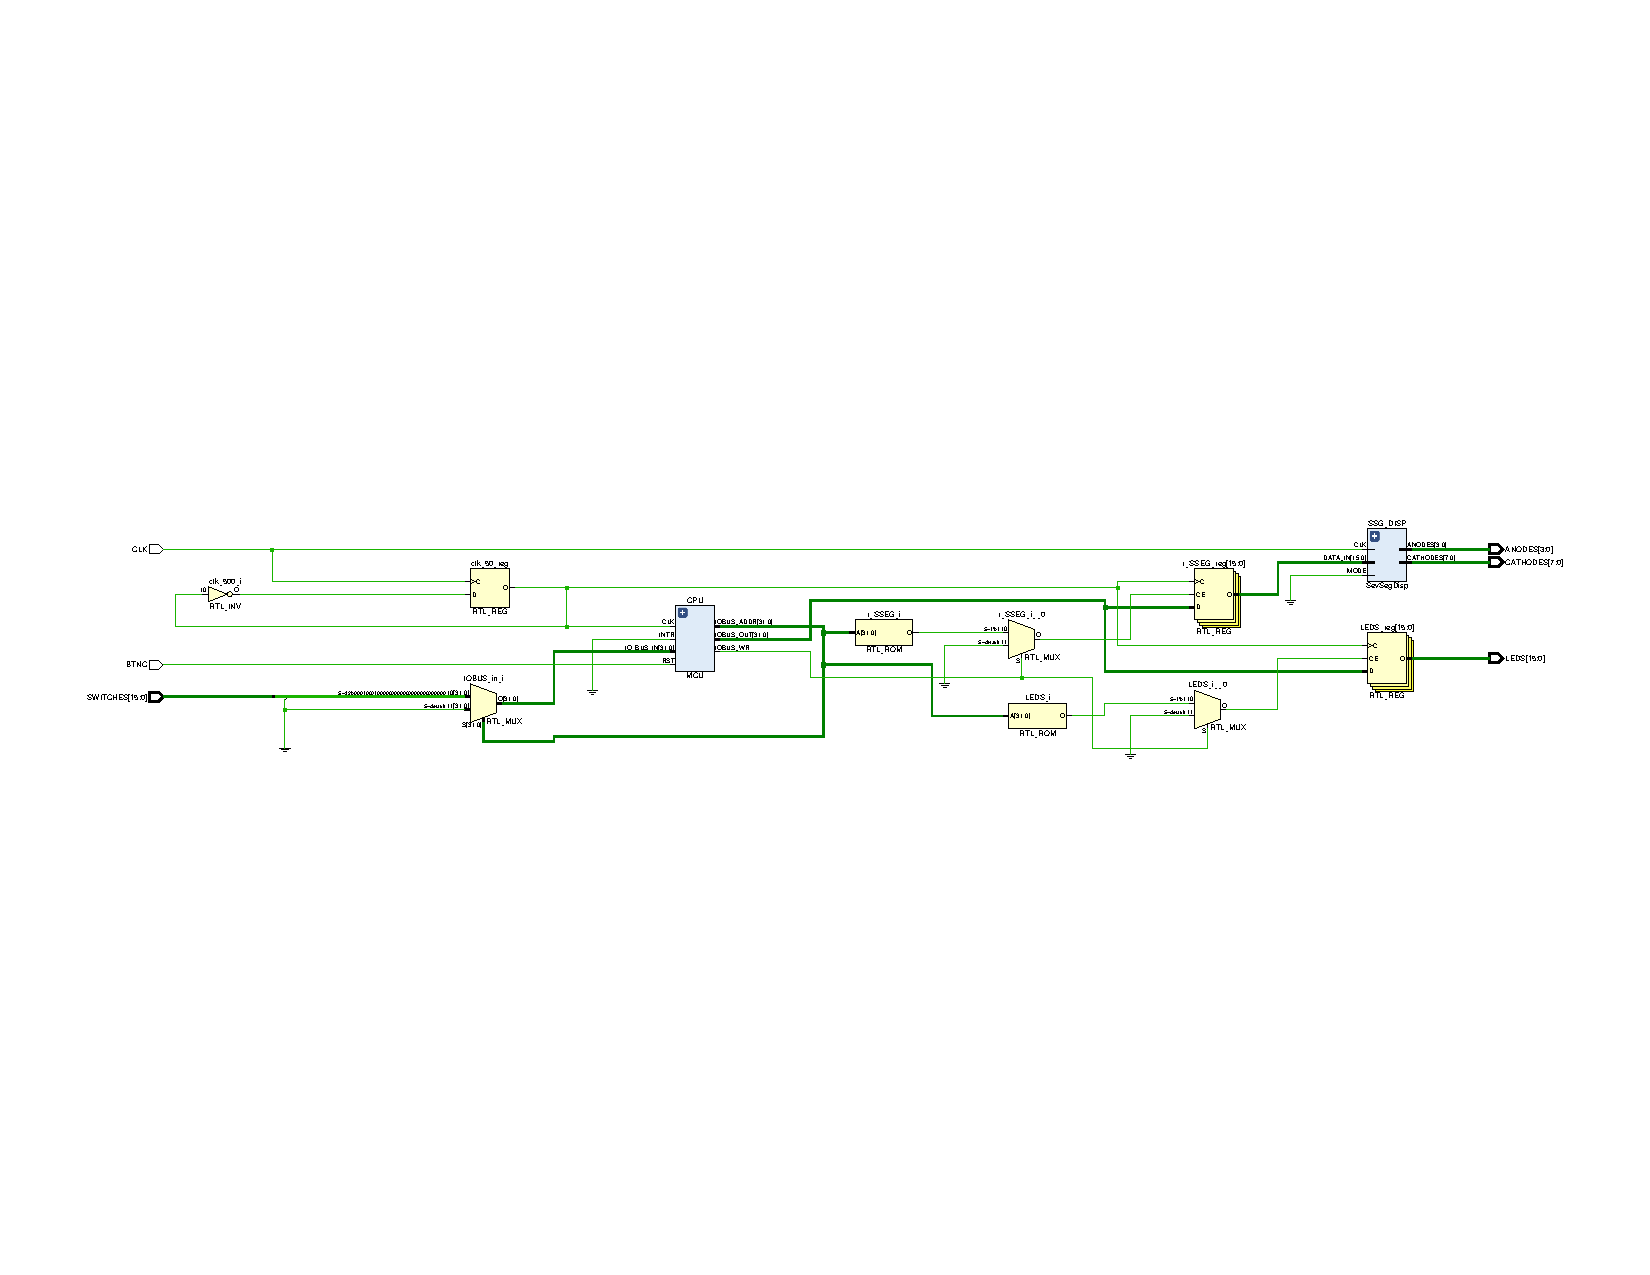
\includegraphics[width=.80\pdfpagewidth]{Figures/wrapperSchematic.pdf}}
    \caption{OTTER MCU Eleborated Design}
    \label{fig:MCUschematic}
\end{figure}

\section{Synthesis Warnings} % Second level section

\subsection{Otter Wrapper Synthesis Warnings} % Third level section
\begin{figure}[H]
    \captionsetup{style=widetable}
    \makebox[.80\pdfpagewidth]{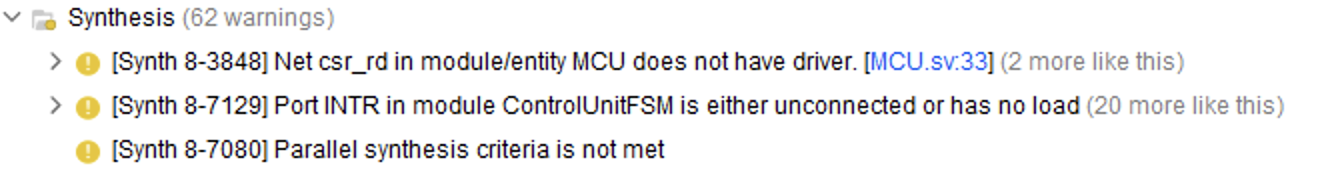
\includegraphics[width=.75\pdfpagewidth]{Figures/Synthesis Warnings.png}}
    \caption{Synthesis Warnings for MCU}
    \label{fig:MCUWarnings}
\end{figure}

The warnings referenced in Figure \ref{fig:MCUWarnings} are not important as there is hardware that will still need to be implemented in future assignments. This means there are various wires that do not have a driver or that do not lead to a defined location. This is fine and in this case does not prevent the design from working. Vivado is simply letting you know that these lines will not be implemented in to the design at this point.

\section{Source Code}
\captionsetup{style=widetable}
% \subsection{Branch Address Generator Source Code} % Third level section

\lstinputlisting[language=Verilog, caption=Control Unit FSM]{/Users/ethanvosburg/Documents/git/CPE-233-Otter/HW6-MCU/MCU/MCU.srcs/sources_1/new/ControlUnitFSM.sv}
\newpage


\lstinputlisting[language=Verilog, caption=Control Unit Decoder]{/Users/ethanvosburg/Documents/git/CPE-233-Otter/HW6-MCU/MCU/MCU.srcs/sources_1/new/ControlUnitDecoder.sv}

% \newpage
% \lstinputlisting[language=Verilog, caption=Master MCU Linking all Modules Together]{/Users/ethanvosburg/Documents/git/CPE-233-Otter/HW6-MCU/MCU/MCU.srcs/sources_1/new/MCU.sv}




\section{Conclusion} % Second level section
\hypersetup{urlcolor=blue} 
In this project, the Otter wrapper was successfully constructed and tested using the provided file \verb|Test_All.mem|. The hardware was found to be functional and it is now ready to be used in projects. While the hardware is not finished, it can be used. In future hardware assignments, interrupts will be added to complete the Otter. 
All code for this assignment can be found \href{https://github.com/EthanV1920/CPE-233-Otter/tree/main}{here}.


\end{fullwidth}

\end{document}